%tex root = thesis.tex

\chapter{Sicherheit}
\label{chapter-Sicherheit}
Für die Sicherheit asymmetrischer Verfahren ist es notwendig, dass die den verschiedenen Verfahren zugrundeliegenden Einwegfunktionen praktisch unumkehrbar sind, da ansonsten aus dem öffentlichen Schlüssel der geheime berechnet werden könnte. Die Sicherheit aller asymmetrischen Kryptosysteme beruht also immer auf unbewiesenen Annahmen, insbesondere auf der Annahme, dass P ungleich NP ist. In der Regel wird von diesen Annahmen jedoch stark vermutet, dass sie zutreffen. Die beim symmetrischen One-Time-Pad erreichbare informationstheoretische Sicherheit kann mit einem asymmetrischen Verfahren nicht erreicht werden, weil ein entsprechend mächtiger Angreifer immer das zugrundeliegende mathematische Problem lösen kann.
\begin{figure*}
	\begin{center}
		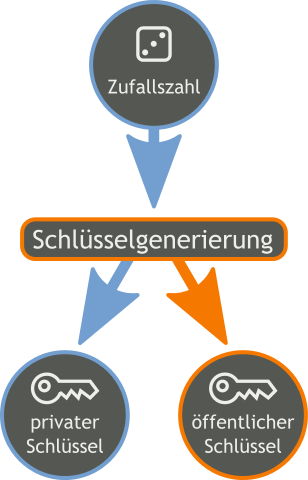
\includegraphics[width=5cm]{abcd.png}	
	\end{center}
	\caption{Erzeugung eines Schlüsselpaars: Blaue Bildelemente sind geheim, orange sind öffentlich.}
	
\end{figure*}

\section{Einwegfunktion}
In der Informatik ist eine Einwegfunktion eine mathematische Funktion, die komplexitätstheoretisch „leicht“ berechenbar, aber „schwer“ umzukehren ist. In einem erweiterten Sinn werden auch Funktionen so bezeichnet, zu denen bisher keine in angemessener Zeit praktisch ausführbare Umkehrung bekannt ist.
Einwegfunktionen bilden die Grundlage asymmetrischer Kryptosysteme.

\section{informationstheoretische Sicherheit}
Perfekte Sicherheit oder auch perfekte Geheimhaltung ist ein von Claude Shannon geprägter Begriff aus der Informationstheorie und Kryptologie. Ein perfekt sicheres Verschlüsselungsverfahren zeichnet sich dadurch aus, dass ein mit ihm erzeugter Schlüsseltext (auch als Geheimtext oder Chiffrat bezeichnet) keinerlei Rückschlüsse auf den korrespondierenden Klartext zulässt. Bei einem solchen Verfahren ist mathematisch bewiesen, dass ein Angreifer, der den Schlüsseltext kennt, abgesehen von der Länge des Klartextes keine weiteren Informationen über diesen gewinnen kann. Er kann den Schlüsseltext also nicht entziffern oder gar das gesamte Verfahren brechen.

\section{RSA-Kryptosystem}
RSA (Rivest, Shamir und Adleman) ist ein asymmetrisches kryptographisches Verfahren, das sowohl zum Verschlüsseln als auch zum digitalen Signieren verwendet werden kann. Es verwendet ein Schlüsselpaar, bestehend aus einem privaten Schlüssel, der zum Entschlüsseln oder Signieren von Daten verwendet wird, und einem öffentlichen Schlüssel, mit dem man verschlüsselt oder Signaturen prüft. Der private Schlüssel wird geheim gehalten und kann nur mit extrem hohem Aufwand aus dem öffentlichen Schlüssel berechnet werden.